

\tikzset{every picture/.style={line width=0.75pt}} %set default line width to 0.75pt        

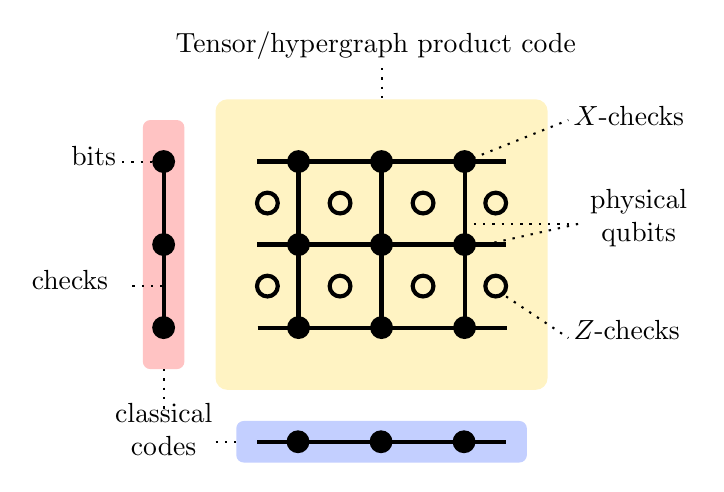
\begin{tikzpicture}[x=0.75pt,y=0.75pt,yscale=-1,xscale=1]
%uncomment if require: \path (0,275); %set diagram left start at 0, and has height of 275

%Rounded Rect [id:dp22143388332555247] 
\draw  [draw opacity=0][fill={rgb, 255:red, 194; green, 206; blue, 255 }  ,fill opacity=0.99 ] (170,228.6) .. controls (170,226.61) and (171.61,225) .. (173.6,225) -- (306.4,225) .. controls (308.39,225) and (310,226.61) .. (310,228.6) -- (310,241.4) .. controls (310,243.39) and (308.39,245) .. (306.4,245) -- (173.6,245) .. controls (171.61,245) and (170,243.39) .. (170,241.4) -- cycle ;
%Rounded Rect [id:dp470208316406618] 
\draw  [draw opacity=0][fill={rgb, 255:red, 255; green, 194; blue, 194 }  ,fill opacity=0.99 ] (125,83.6) .. controls (125,81.61) and (126.61,80) .. (128.6,80) -- (141.4,80) .. controls (143.39,80) and (145,81.61) .. (145,83.6) -- (145,196.4) .. controls (145,198.39) and (143.39,200) .. (141.4,200) -- (128.6,200) .. controls (126.61,200) and (125,198.39) .. (125,196.4) -- cycle ;
%Rounded Rect [id:dp03513935583523131] 
\draw  [draw opacity=0][fill={rgb, 255:red, 255; green, 243; blue, 194 }  ,fill opacity=0.99 ] (160,75.75) .. controls (160,72.58) and (162.58,70) .. (165.75,70) -- (314.25,70) .. controls (317.42,70) and (320,72.58) .. (320,75.75) -- (320,204.25) .. controls (320,207.42) and (317.42,210) .. (314.25,210) -- (165.75,210) .. controls (162.58,210) and (160,207.42) .. (160,204.25) -- cycle ;
%Straight Lines [id:da7185026143243305] 
\draw [line width=1.5]    (180,100) -- (300,100) ;
%Straight Lines [id:da8313570524380964] 
\draw [line width=1.5]    (180,140) -- (300,140) ;
%Straight Lines [id:da9953047772585519] 
\draw [line width=1.5]    (200,100) -- (200,180) ;
%Straight Lines [id:da6537085237341653] 
\draw [line width=1.5]    (240,100) -- (240,180) ;
%Straight Lines [id:da4083149661642169] 
\draw [line width=1.5]    (280,100) -- (280,185) ;
%Straight Lines [id:da7864030630152321] 
\draw [line width=1.5]    (180.25,180) -- (189.75,180) -- (300.25,180) ;
%Shape: Circle [id:dp9396697829244669] 
\draw  [fill={rgb, 255:red, 0; green, 0; blue, 0 }  ,fill opacity=1 ] (195,100) .. controls (195,97.24) and (197.24,95) .. (200,95) .. controls (202.76,95) and (205,97.24) .. (205,100) .. controls (205,102.76) and (202.76,105) .. (200,105) .. controls (197.24,105) and (195,102.76) .. (195,100) -- cycle ;
%Shape: Circle [id:dp2777712322207504] 
\draw  [fill={rgb, 255:red, 0; green, 0; blue, 0 }  ,fill opacity=1 ] (235,100) .. controls (235,97.24) and (237.24,95) .. (240,95) .. controls (242.76,95) and (245,97.24) .. (245,100) .. controls (245,102.76) and (242.76,105) .. (240,105) .. controls (237.24,105) and (235,102.76) .. (235,100) -- cycle ;
%Shape: Circle [id:dp9770309094107599] 
\draw  [fill={rgb, 255:red, 0; green, 0; blue, 0 }  ,fill opacity=1 ] (275,100) .. controls (275,97.24) and (277.24,95) .. (280,95) .. controls (282.76,95) and (285,97.24) .. (285,100) .. controls (285,102.76) and (282.76,105) .. (280,105) .. controls (277.24,105) and (275,102.76) .. (275,100) -- cycle ;
%Shape: Circle [id:dp0007255817041109669] 
\draw  [fill={rgb, 255:red, 0; green, 0; blue, 0 }  ,fill opacity=1 ] (195,140) .. controls (195,137.24) and (197.24,135) .. (200,135) .. controls (202.76,135) and (205,137.24) .. (205,140) .. controls (205,142.76) and (202.76,145) .. (200,145) .. controls (197.24,145) and (195,142.76) .. (195,140) -- cycle ;
%Shape: Circle [id:dp22755606896736325] 
\draw  [fill={rgb, 255:red, 0; green, 0; blue, 0 }  ,fill opacity=1 ] (235,140) .. controls (235,137.24) and (237.24,135) .. (240,135) .. controls (242.76,135) and (245,137.24) .. (245,140) .. controls (245,142.76) and (242.76,145) .. (240,145) .. controls (237.24,145) and (235,142.76) .. (235,140) -- cycle ;
%Shape: Circle [id:dp35741023769095337] 
\draw  [fill={rgb, 255:red, 0; green, 0; blue, 0 }  ,fill opacity=1 ] (275,140) .. controls (275,137.24) and (277.24,135) .. (280,135) .. controls (282.76,135) and (285,137.24) .. (285,140) .. controls (285,142.76) and (282.76,145) .. (280,145) .. controls (277.24,145) and (275,142.76) .. (275,140) -- cycle ;
%Shape: Circle [id:dp5745096142293205] 
\draw  [fill={rgb, 255:red, 0; green, 0; blue, 0 }  ,fill opacity=1 ] (195,180) .. controls (195,177.24) and (197.24,175) .. (200,175) .. controls (202.76,175) and (205,177.24) .. (205,180) .. controls (205,182.76) and (202.76,185) .. (200,185) .. controls (197.24,185) and (195,182.76) .. (195,180) -- cycle ;
%Shape: Circle [id:dp54039886697822] 
\draw  [fill={rgb, 255:red, 0; green, 0; blue, 0 }  ,fill opacity=1 ] (235,180) .. controls (235,177.24) and (237.24,175) .. (240,175) .. controls (242.76,175) and (245,177.24) .. (245,180) .. controls (245,182.76) and (242.76,185) .. (240,185) .. controls (237.24,185) and (235,182.76) .. (235,180) -- cycle ;
%Shape: Circle [id:dp10040664716660697] 
\draw  [fill={rgb, 255:red, 0; green, 0; blue, 0 }  ,fill opacity=1 ] (275,180) .. controls (275,177.24) and (277.24,175) .. (280,175) .. controls (282.76,175) and (285,177.24) .. (285,180) .. controls (285,182.76) and (282.76,185) .. (280,185) .. controls (277.24,185) and (275,182.76) .. (275,180) -- cycle ;
%Shape: Circle [id:dp2682894278787049] 
\draw  [line width=1.5]  (215,120) .. controls (215,117.24) and (217.24,115) .. (220,115) .. controls (222.76,115) and (225,117.24) .. (225,120) .. controls (225,122.76) and (222.76,125) .. (220,125) .. controls (217.24,125) and (215,122.76) .. (215,120) -- cycle ;
%Shape: Circle [id:dp8966595793927485] 
\draw  [line width=1.5]  (255,120) .. controls (255,117.24) and (257.24,115) .. (260,115) .. controls (262.76,115) and (265,117.24) .. (265,120) .. controls (265,122.76) and (262.76,125) .. (260,125) .. controls (257.24,125) and (255,122.76) .. (255,120) -- cycle ;
%Shape: Circle [id:dp8886077713077252] 
\draw  [line width=1.5]  (215,160) .. controls (215,157.24) and (217.24,155) .. (220,155) .. controls (222.76,155) and (225,157.24) .. (225,160) .. controls (225,162.76) and (222.76,165) .. (220,165) .. controls (217.24,165) and (215,162.76) .. (215,160) -- cycle ;
%Shape: Circle [id:dp4297496569136454] 
\draw  [line width=1.5]  (255,160) .. controls (255,157.24) and (257.24,155) .. (260,155) .. controls (262.76,155) and (265,157.24) .. (265,160) .. controls (265,162.76) and (262.76,165) .. (260,165) .. controls (257.24,165) and (255,162.76) .. (255,160) -- cycle ;
%Straight Lines [id:da6946255251193814] 
\draw [line width=1.5]    (135,100) -- (135,180) ;
%Shape: Circle [id:dp2862743840664752] 
\draw  [fill={rgb, 255:red, 0; green, 0; blue, 0 }  ,fill opacity=1 ] (130,100) .. controls (130,97.24) and (132.24,95) .. (135,95) .. controls (137.76,95) and (140,97.24) .. (140,100) .. controls (140,102.76) and (137.76,105) .. (135,105) .. controls (132.24,105) and (130,102.76) .. (130,100) -- cycle ;
%Shape: Circle [id:dp06319104540768339] 
\draw  [fill={rgb, 255:red, 0; green, 0; blue, 0 }  ,fill opacity=1 ] (130,140) .. controls (130,137.24) and (132.24,135) .. (135,135) .. controls (137.76,135) and (140,137.24) .. (140,140) .. controls (140,142.76) and (137.76,145) .. (135,145) .. controls (132.24,145) and (130,142.76) .. (130,140) -- cycle ;
%Shape: Circle [id:dp8917628215544027] 
\draw  [fill={rgb, 255:red, 0; green, 0; blue, 0 }  ,fill opacity=1 ] (130,180) .. controls (130,177.24) and (132.24,175) .. (135,175) .. controls (137.76,175) and (140,177.24) .. (140,180) .. controls (140,182.76) and (137.76,185) .. (135,185) .. controls (132.24,185) and (130,182.76) .. (130,180) -- cycle ;
%Straight Lines [id:da9878368991357702] 
\draw  [dash pattern={on 0.84pt off 2.51pt}]  (115,100) -- (130,100) ;
%Straight Lines [id:da48285493465469065] 
\draw  [dash pattern={on 0.84pt off 2.51pt}]  (120,160) -- (135,160) ;
%Straight Lines [id:da5818415971249424] 
\draw  [dash pattern={on 0.84pt off 2.51pt}]  (280,100) -- (330,80) ;
%Straight Lines [id:da32466921044761854] 
\draw  [dash pattern={on 0.84pt off 2.51pt}]  (300,165) -- (330,185) ;
%Straight Lines [id:da40657015888893877] 
\draw  [dash pattern={on 0.84pt off 2.51pt}]  (290,140) -- (335,130) ;
%Straight Lines [id:da20859695153194213] 
\draw  [dash pattern={on 0.84pt off 2.51pt}]  (280,130) -- (335,130) ;
%Straight Lines [id:da6822142544403822] 
\draw  [dash pattern={on 0.84pt off 2.51pt}]  (135,200) -- (135,220) ;
%Straight Lines [id:da03323895635752949] 
\draw  [dash pattern={on 0.84pt off 2.51pt}]  (160,235) -- (170,235) ;
%Straight Lines [id:da2805464127859385] 
\draw  [dash pattern={on 0.84pt off 2.51pt}]  (240,55) -- (240,70) ;
%Straight Lines [id:da5067552483919655] 
\draw [line width=1.5]    (180,235) -- (189.5,235) -- (300,235) ;
%Shape: Circle [id:dp361674319320721] 
\draw  [fill={rgb, 255:red, 0; green, 0; blue, 0 }  ,fill opacity=1 ] (194.75,235) .. controls (194.75,232.24) and (196.99,230) .. (199.75,230) .. controls (202.51,230) and (204.75,232.24) .. (204.75,235) .. controls (204.75,237.76) and (202.51,240) .. (199.75,240) .. controls (196.99,240) and (194.75,237.76) .. (194.75,235) -- cycle ;
%Shape: Circle [id:dp14935624369602674] 
\draw  [fill={rgb, 255:red, 0; green, 0; blue, 0 }  ,fill opacity=1 ] (234.75,235) .. controls (234.75,232.24) and (236.99,230) .. (239.75,230) .. controls (242.51,230) and (244.75,232.24) .. (244.75,235) .. controls (244.75,237.76) and (242.51,240) .. (239.75,240) .. controls (236.99,240) and (234.75,237.76) .. (234.75,235) -- cycle ;
%Shape: Circle [id:dp5448923044982008] 
\draw  [fill={rgb, 255:red, 0; green, 0; blue, 0 }  ,fill opacity=1 ] (274.75,235) .. controls (274.75,232.24) and (276.99,230) .. (279.75,230) .. controls (282.51,230) and (284.75,232.24) .. (284.75,235) .. controls (284.75,237.76) and (282.51,240) .. (279.75,240) .. controls (276.99,240) and (274.75,237.76) .. (274.75,235) -- cycle ;
%Shape: Circle [id:dp8778336468318328] 
\draw  [line width=1.5]  (290,120) .. controls (290,117.24) and (292.24,115) .. (295,115) .. controls (297.76,115) and (300,117.24) .. (300,120) .. controls (300,122.76) and (297.76,125) .. (295,125) .. controls (292.24,125) and (290,122.76) .. (290,120) -- cycle ;
%Shape: Circle [id:dp9087440034913905] 
\draw  [line width=1.5]  (290,160) .. controls (290,157.24) and (292.24,155) .. (295,155) .. controls (297.76,155) and (300,157.24) .. (300,160) .. controls (300,162.76) and (297.76,165) .. (295,165) .. controls (292.24,165) and (290,162.76) .. (290,160) -- cycle ;
%Shape: Circle [id:dp9078486972487199] 
\draw  [line width=1.5]  (180,160) .. controls (180,157.24) and (182.24,155) .. (185,155) .. controls (187.76,155) and (190,157.24) .. (190,160) .. controls (190,162.76) and (187.76,165) .. (185,165) .. controls (182.24,165) and (180,162.76) .. (180,160) -- cycle ;
%Shape: Circle [id:dp38296270902884433] 
\draw  [line width=1.5]  (180,120) .. controls (180,117.24) and (182.24,115) .. (185,115) .. controls (187.76,115) and (190,117.24) .. (190,120) .. controls (190,122.76) and (187.76,125) .. (185,125) .. controls (182.24,125) and (180,122.76) .. (180,120) -- cycle ;

% Text Node
\draw (136,36) node [anchor=north west][inner sep=0.75pt]   [align=left] {\begin{minipage}[lt]{149.58912pt}\setlength\topsep{0pt}
\begin{center}
Tensor/hypergraph product code
\end{center}

\end{minipage}};
% Text Node
\draw (106,215) node [anchor=north west][inner sep=0.75pt]   [align=left] {\begin{minipage}[lt]{41.267500000000005pt}\setlength\topsep{0pt}
\begin{center}
classical\\codes
\end{center}

\end{minipage}};
% Text Node
\draw (89,91) node [anchor=north west][inner sep=0.75pt]   [align=left] {bits};
% Text Node
\draw (70,151) node [anchor=north west][inner sep=0.75pt]   [align=left] {checks};
% Text Node
\draw (331,72) node [anchor=north west][inner sep=0.75pt]   [align=left] {$\displaystyle X$-checks};
% Text Node
\draw (331,175) node [anchor=north west][inner sep=0.75pt]   [align=left] {$\displaystyle Z$-checks};
% Text Node
\draw (336,112) node [anchor=north west][inner sep=0.75pt]   [align=left] {\begin{minipage}[lt]{39.578108pt}\setlength\topsep{0pt}
\begin{center}
physical\\qubits
\end{center}

\end{minipage}};


\end{tikzpicture}
